\section{Internet of Plants}

\subsection{Overview}

The Internet of Plants, also called IoP, is a concept that aims to interconnect the plant device previously built.
This in order to empower the device capabilities and to provide a better user experience.
This project includes:
\begin{itemize}
    \item A better sound quality by using professional sonification software
    \item The ability to create a full artistic experience by creating a distributed instrument
    \item Refining the interaction with the plant by using more complex data analyses
\end{itemize}



\subsection{Communication}

The communication system is based on WiFi technology. The ESP32 has specific wireless capabilities.
The server and the ESP32 devices are connected to the same network.
The ESP32 sends the raw data to the server using IP\footnote{Internet Protocol}. This is done
through a TCP \footnote{Transmission Control Protocol} socket open between the server and one ESP32.
The server can open as many socket as there are clients. The data sent using a string.
A "#" start character and a ";\\n" stop character are used to prevent the messages to 
be truncated and still processed on the server side. The IP protocol (whether it is on WiFi
or Ethernet) has been chosen for this application for several reasons:

\begin{itemize}
    \item Allow high bandwidth
    \item Available in most places
    \item Allow connection of multiple devices
    \item Already available on the server and on the ESP32
\end{itemize}

Other communication protocols have been benchmarked. Here is a table that summarizes
the choice: 

\begin{table}[]
    \begin{tabular}{|l|l|l|l|l|}
    \hline
    Protocol                            & IP   & Bluetooth & BLE   & Zigbee \\ \hline
    Handle multiple connections         & Yes  & No        & No    & Yes    \\
    Requires additional hardware        & No   & No        & No    & Yes    \\
    Subject to interference             & Yes  & Few       & Few   & Yes    \\
    Energy efficiency (using a battery) & Days & Months    & Years & Years  \\ \hline
    \end{tabular}
    \caption{Comparison between different communication protocol to find the one that will suits our needs the best.}
    \label{tab:protocol_comparison}
\end{table}

The result of this table confirms that WiFi is the right choice for our specific application.
\subsection{Server}

The server is a small fanless computer running Lubuntu. Lubuntu is a lighter version of Ubuntu
that includes LXQt as desktop environnement. The choice of a distribution with graphical
interface is induced by the use of \textit{Pure Data} as sonification software.

Pure Data (PD) is an open-source visual programming language designed primarily for 
creating interactive multimedia applications, particularly in the fields of audio, video, 
and graphical processing.
Pure Data is part of a family of patcher programming languages, which also includes Max/MSP.
Unlike traditional text-based programming, PD uses a graphical interface where users connect 
"objects" with virtual patch cables to create complex data flows and signal processing chains. 
Its modular design allows for real-time manipulation of sound and graphics, making it a powerful 
tool for artists, musicians, and researchers interested in exploring experimental media. 

Pure Data requires, in a development environnement, a graphical interface to test and debug.
The Pure Data patch receive the data through a TCP socket. The data is processed through several 
operations. Then, if a threshold is passed, an interaction happened and the music is triggered.
The music is outputted through the item \textit{DAC} which means Digital to Analog Converter. 
The digital input from pure data is converted to a sound that speakers can output.

\begin{figure}[h]
    \centering
    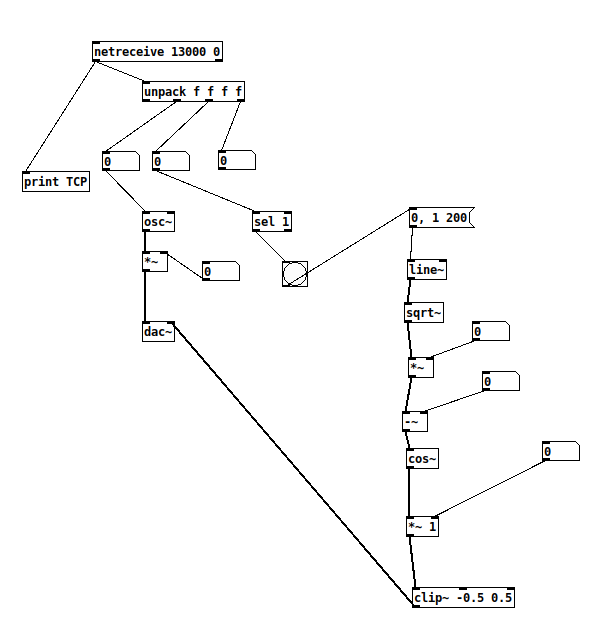
\includegraphics[width=\textwidth]{pure_data_patch.png}
    \caption{Basic \textit{Pure Data} patch that is used for sonification of the data
    of the plant. In case of an art exhibition, the Pure Data patch can be upgraded to meet the
    artist needs} 
    \vspace{0.1cm}
    \label{fig:pure_data_patch}
\end{figure}


Pure Data is a sonification software that require data as input. In order to get and process the data,
we designed a Python based software. %FIXME: microservices
The software is object oriented. The standalone IoP modules connect using WiFi to the receiver module
of the software. The connection is made using TCP socket from the ESP32 to the server.
The main module of the software then creates software abstraction of the standalone module. 
The abstraction module is processing and storing all the processed data.
The main module then send the processed data to Pure Data patch using also local TCP socket.

\begin{figure}[h]
    \centering
    \includegraphics[width=\textwidth]{iop_architecture.png}
    \caption{Architecture diagram of Internet of Plants project centered on server-side.} 
    \vspace{0.1cm}
    \label{fig:server_architecture}
\end{figure}


\subsection{Deployment} %and application}

The server software is easily deployable. The software includes a shell script to deploy the server service.
Indeed, the server relies on a \textit{systemd} linux service. \textit{Systemd} \cite{Both2020} is a
Linux software that manage application that runs \textit{daemons} or services.
\textit{Daemons} are pieces of software that run in background of the operating
system. They are mainly started at the during the boot of the operating system.

The server is deployed that way so the software starts with the operating system.
It waits for the network interfaces to be up and running and opens the socket.
The installation tool install Python dependencies, fill in the templated service file,
install the service and enable it. The server is able to receive data from IoP standalone
modules and use Pure Data software for sonification. The last step is to connect
a jack speaker to the jack builtin output.

On the IoP standalone module side, it requires a software that is able to upload 
firmware to an ESP32 MCU. I recommend using PlatformIO which is an open source 
embedded software development platform. The firmware is developed using this platform.
The source code is written in C++ using the Arduino framework. You flash the firmware
to the chip after setting up the WiFi credentials.
The module sends all the retrieved data to the server.

\subsubsection{Distributed instruments}

This IoP architecture enables possibilities on deploying a distributed instrument.
It is possible to deploy several IoP standalone modules, in different plants and build a entire musical instrument.
Modules reach out to the server and the server link an ID to the different connected devices.
The data is sent to Pure Data and using the software, you can create many sounds depending on the 
module (and thus plant) origin. Pure Data offers a fine control over pitch, sound, rhythm, tone and much more.

\subsection{output}

\subsubsection{Art exhibition}

To push further the distributed instrument, it is possible to build an entire 
musical experience for an art exhibition.
The immersive experience can take place as a fully connected forest. The music would vary
depending on the touch interaction that people have with the plants.

\begin{figure}[h!]
    \centering
    \includegraphics[width=\textwidth]{art_exhibition.pdf}
    \caption{Schematic of the IoP art exhibition. The music varies depending on the 
    interaction that people have with the installation. People are immersed into the full
    musical and sonification experience.} 
    \vspace{0.1cm}
    \label{fig:art_exhibition}
\end{figure}

This exhibition could allow people to rethink the way the see and interact with plants.
Plants are not seen anymore as decoration object but as a living being.
The living being is here highlighted by the fact that plants can now express their state.
The humidity level, the light intensity and other state signs are modifying the plant 
reaction.


Musicians can also work in pair with plants to create songs using music from the plants.
The music coming from the plant is fully configurable with the sonification software.


\subsubsection{Final product, limitations and future work}

Final product is a software that allows the connection between multiple standalone IoP modules and a sonification
software, Pure Data. The software handle multiple connection and apply a filtering and cleaning on the data 
retrieved. The data is then sent to Pure Data for sonification.

\begin{figure}[h!]
    \centering
    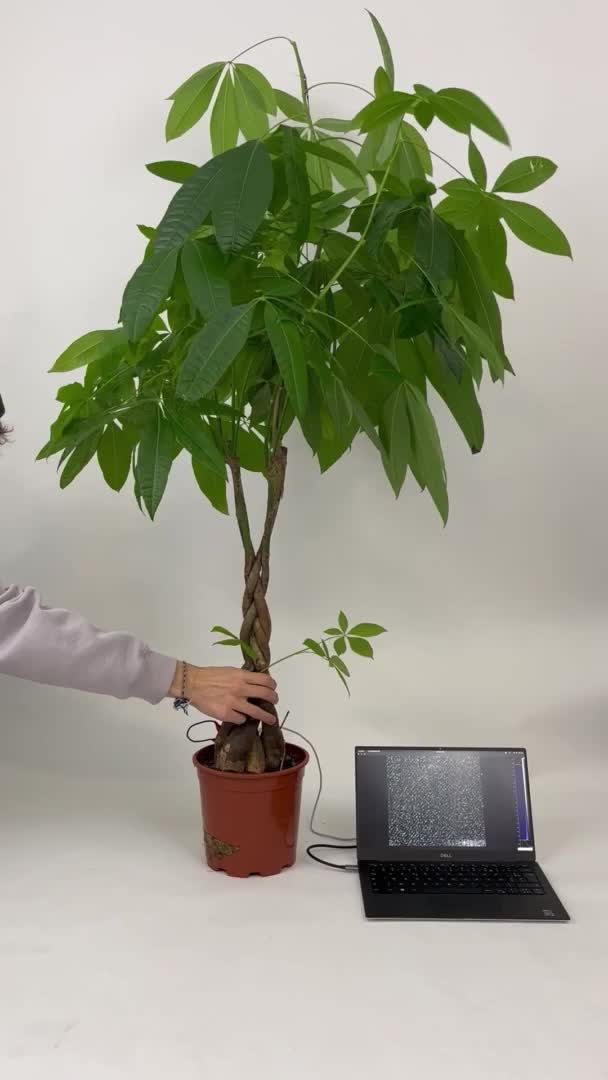
\includegraphics[width=0.8\textwidth]{images/standalone_demo.jpg}
    \caption{Server-module demo. In this specific use case, the module is connected by wire to a computer.
    Otherwise, the module is usable wirelessly. 
    The computer is acting as a server.
    On this version of the demo, the screen is displaying a figure that is evolving depending on the touch interaction.
    The computer, acting as the server, is producing the sound using Pure Data software.} 
    \vspace{0.1cm}
    \label{fig:standalone_demo}
\end{figure}

On the limitation side, the use of WiFi ease a lot the deployment of the system, however 
% TODO: Talk about overcrowded wifi
% talk about frame dropped and lost. 
% Talk about the start and stop tag to check if frame is entire

\subsection{Conclusion}

